\documentclass[a4paper,12pt,oneside,pdflatex,italian,final,twocolumn]{article}

%\documentclass[a4paper,12pt,oneside,pdflatex,italian,final,twocolumn]{article}
%\documentclass[a4paper,11pt,oneside,openany]{memoir} 	% Openright aabner kapitler paa hoejresider (openany = vilkaarlig/begge)


%%%% PAKKER %%%%
% ¤¤ Oversaettelse og tegnsaetning ¤¤ %
\usepackage[utf8]{inputenc}					% Input-indkodning af tegnsaet, dvs. input fra keyboard, tegnoversigt eller andet (UTF8 = Unicode)
\usepackage[T1]{fontenc}					% Output-indkodning af tegnsaet, dvs. printede fonte og tegn (T1 = Type 1 font med support for de fleste europaeiske sprog)
%\usepackage[danish]{babel}					% Sproglig fremstilling af elementer (figur vs. figure, litteratur vs. bibliography osv.)
\usepackage{csquotes}

\usepackage{booktabs}

\usepackage{changepage}

\usepackage{ragged2e,anyfontsize}			% Justering af elementer
\usepackage{lastpage}

% ¤¤ Figurer og tabeller (floats) ¤¤ %
\usepackage{graphicx} 						% Inkludering af eksterne billeder (JPG, PNG, PDF)
\usepackage{multirow}
\usepackage{multicol}% Fletning af raekker og kolonner (\multicolumn og \multirow)
\usepackage{colortbl} 						% Farver i tabeller (fx \columncolor, \rowcolor og \cellcolor)
\usepackage[dvipsnames, svgnames, table]{xcolor}        		% Definer farver med \definecolor. Se mere: http://en.wikibooks.org/wiki/LaTeX/Colors
\usepackage{flafter}						% Soerger for, at floats ikke optraeder i teksten foer deres reference
\usepackage{float}							% Muliggoer eksakt placering af floats, fx \begin{figure}[H]
\let\newfloat\relax 						% Justering mellem float-pakken og memoir
%\usepackage{eso-pic}						% Tilfoej billedekommandoer paa hver side
\usepackage{wrapfig}						% Indsaettelse af figurer omsvoebt af tekst 
%\usepackage{multicol}         	        	% Muliggoer tekst i spalter
%\usepackage{rotating}						% Rotation af tekst med \begin{sideways}...\end{sideways}
\usepackage{gensymb}
% nogle andre ting til tabeller
\renewcommand{\arraystretch}{1.5}           % Højde for hver celle
\setlength{\arrayrulewidth}{0.5mm}          % Tykkelse af streger i tabeller
\arrayrulecolor[HTML]{9B9B9B}               % Farve til streger i tabeller

% nogle ting til grafer
\usepackage{pgfplots}                       % Til at plotte grafer, Tikz baseret
    \pgfplotsset{width=10cm,compat=1.9}
\usepackage{tikz}
\usetikzlibrary{fit,backgrounds}
\usetikzlibrary{calc}
\usetikzlibrary{positioning}
\usetikzlibrary{shapes.geometric}

% ¤¤ Matematik mm. ¤¤
\usepackage{amsmath,amssymb,stmaryrd} 		% Avancerede matematik-udvidelser
\usepackage{mathtools}% Andre matematik- og tegnudvidelser
\usepackage{bm} %Matematisk fed skrift
\usepackage{mathrsfs}
\usepackage{textcomp}                 		% Symbol-udvidelser (fx promille-tegn med \textperthousand)
\usepackage{siunitx}						% Flot og konsistent praesentation af tal og enheder med \si{enhed} og \SI{tal}{enhed}
\sisetup{output-decimal-marker = {.}}		% Opsaetning af \SI og decimalseparator
\sisetup{group-separator = \ }
\sisetup{output-exponent-marker=\ensuremath{\mathrm{E}}}
\DeclareSIUnit{\flow}{flow}
\DeclareSIUnit{\frame}{frame}
\DeclareSIUnit{\degree}{deg}
\DeclareSIUnit{\baud}{Baud}


\usepackage{icomma}                         % Komma som decimalseperator fix
\usepackage{makecell}


% ¤¤ Referencer og kilder ¤¤ %
\usepackage{varioref}				% Muliggoer bl.a. krydshenvisninger med sidetal (\vref)
						% Udvidelse med naturvidenskabelige citationsmodeller, herunder Harvard-modellen


% ¤¤ Misc. ¤¤ %
\usepackage{listings}						
% Placer kildekode i dokumentet med \begin{lstlisting}...\end{lstlisting}
\usepackage{lipsum}							
% Dummy tekst med fx \lipsum[2]
\usepackage[shortlabels]{enumitem}			
% Muliggoer enkelt konfiguration af lister (se \setlist nedenfor)
\usepackage{pdfpages}						
% Goer det muligt at inkludere pdf-dokumenter med kommandoen \includepdf[pages={x-y}]{fil.pdf}	
\pdfoptionpdfminorversion=6					
% Muliggoer inkludering af pdf-dokumenter af version 1.6 og hoejere
%\pretolerance=2500 							
% Justering af afstand mellem ord (hoejt tal, mindre orddeling og mere luft mellem ord)

% Kommentarer og rettelser med \fxnote. Med 'final' i stedet for 'draft' udloeser hver note en error i den faerdige rapport.
\usepackage[footnote,draft,danish,silent,nomargin]{fixme}		

\usepackage{subcaption}

\usepackage{longtable} %makes it so tables can fill multiple pages

%%%% BRUGERDEFINEREDE INDSTILLINGER %%%%

% ¤¤ Marginer ¤¤ %
%\setlrmarginsandblock{3cm}{3cm}{*}		% \setlrmarginsandblock{Indbinding}{Kant}{Ratio}
%\setlrmarginsandblock{2.5cm}{2.5cm}{*}		%
%\setulmarginsandblock{3cm}{3.0cm}{*}		% \setulmarginsandblock{Top}{Bund}{Ratio}
%\checkandfixthelayout 						
% Oversaetter vaerdier til brug for andre pakker
%	¤¤ Afsnitsformatering ¤¤ %
\setlength{\parindent}{0mm}           		
% Stoerrelse af indryk
\setlength{\parskip}{3mm}          			
% Afstand mellem afsnit ved brug af double Enter
\linespread{1,1}							
% Linjeafstand

% ¤¤ Litteraturlisten ¤¤ %

\usepackage[
%  disable, %turn off todonotes
  colorinlistoftodos, %enable a coloured square in the list of todos
  textwidth=\marginparwidth, %set the width of the todonotes
  textsize=scriptsize, %size of the text in the todonotes
  ]{todonotes}



% ¤¤ Dybde af overskrifter ¤¤ %
%\setsecnumdepth{subsection}		 			
% Dybden af nummerede overkrifter (part/chapter/section/subsection)
% Dybden af overskrifter vist i indholdsfortegnelsen


% ¤¤ Lister ¤¤ %
\setlist{
  topsep=0pt,								
  % Vertikal afstand mellem tekst og listen
  itemsep=-1ex,								
  % Vertikal afstand mellem items
} 

% ¤¤ Visuelle referencer ¤¤ %
\usepackage[colorlinks]{hyperref}			
% Danner klikbare referencer (hyperlinks) i dokumentet
\hypersetup{colorlinks = true,				
% Opsaetning af farvede hyperlinks (interne links, citeringer og URL)
    linkcolor = black,
    citecolor = black,
    urlcolor = black
}


% ¤¤ Opsaetning af figur- og tabeltekst ¤¤ %
%\captionnamefont{\small\bfseries\itshape}	
% Opsaetning af tekstdelen ('Figur' eller 'Tabel')
%\captiontitlefont{\small}					
% Opsaetning af nummerering
%\captiondelim{. }							
% Seperator mellem nummerering og figurtekst
%\captionstyle{\centering}					
% Justering/placering af figurteksten (centreret = \centering, venstrejusteret = \raggedright)

%\captionwidth{1\linewidth}					
% Bredden af figurteksten
%\hangcaption								
% Venstrejusterer fler-linjers figurtekst under hinanden
\setlength{\belowcaptionskip}{0pt}			
% Afstand under figurteksten

% ¤¤ Opsaetning af listings ¤¤ %
%Se særskillet dokument. 
%
\definecolor{commentGreen}{RGB}{34,139,24}
\definecolor{stringPurple}{RGB}{208,76,239}
\colorlet{keyword}{blue!100!black!80}
\colorlet{comment}{green!60!black!100}



\lstset{language=Matlab,					% Sprog
	basicstyle=\ttfamily\scriptsize,		% Opsaetning af teksten
	keywords={for,if,while,else,elseif,		% Noegleord at fremhaeve
			  end,break,return,case,
			  switch,function},
	keywordstyle=\color{blue},				% Opsaetning af noegleord
	commentstyle=\color{commentGreen},		% Opsaetning af kommentarer
	stringstyle=\color{stringPurple},		% Opsaetning af strenge
	showstringspaces=false,					% Mellemrum i strenge enten vist eller blanke
	numbers=left, numberstyle=\tiny,		% Linjenumre
	extendedchars=true, 					% Tillader specielle karakterer
	columns=flexible,						% Kolonnejustering
	breaklines, breakatwhitespace=true,		% Bryd lange linjer
}

\lstdefinelanguage{VHDL}{
    %alt blåt
  morekeywords=[1]{
    library,use,all,entity,is,port,in,out,end,architecture,of,
    begin,and, AND, or, OR, Not, not, NOT, downto,ALL, PORT, to, process, if, elsif, else, signal, Integer, loop, for, return, function, variable, Component, case, when, others, then, null 
  },
  %alt lyserødt (bordeaux rød?)
  morekeywords=[2]{
    STD_LOGIC_VECTOR,STD_LOGIC,IEEE,STD_LOGIC_1164,
    NUMERIC_STD,STD_LOGIC_ARITH,STD_LOGIC_UNSIGNED,std_logic_vector,
    std_logic, STD_LOGIC_1164, numeric_std,to_unsigned,andOrVectors
  },
  morecomment=[l]--,
  morecomment=[s][\color{codegray}]{"}{"}
}
\lstset{language=VHDL,texcl=true}

\lstdefinestyle{vhdl}{
  language     = VHDL,
  basicstyle   = \footnotesize \ttfamily,
  keywordstyle = [1]\color{keyword}\bfseries,
  keywordstyle = [2]\color{stringPurple}\bfseries,
  commentstyle = \color{comment},
  tabsize=3		                   % sets default tabsize to 2 spaces
}


\definecolor{Python:commentGreen}{RGB}{34,139,24}
\definecolor{Python:stringPurple}{RGB}{208,76,239}
\colorlet{Python:keyword}{blue!100!black!80}
\colorlet{Python:comment}{green!60!black!100}



\lstdefinelanguage{python}{
    %alt blåt
  morekeywords=[1]{
    access,and,break,class,continue,def,del,elif,else,except,exec,finally,for,from,global,if,import,in,is,lambda,not,or,pass,print,raise,return,try,while
  },
  %alt lyserødt (bordeaux rød?)
  morekeywords=[2]{
    abs,all,any,basestring,bin,bool,bytearray,callable,chr,classmethod,cmp,compile,complex,delattr,dict,dir,divmod,enumerate,eval,execfile,file,filter,float,format,frozenset,getattr,globals,hasattr,hash,help,hex,id,input,int,isinstance,issubclass,iter,len,list,locals,long,map,max,memoryview,min,next,object,oct,open,ord,pow,property,range,raw_input,reduce,reload,repr,reversed,round,set,setattr,slice,sorted,staticmethod,str,sum,super,tuple,type,unichr,unicode,vars,xrange,zip,apply,buffer,coerce,intern
  },
  morecomment=[l]\#,
  morecomment=[s][\color{codegray}]{"}{"}
}
\lstset{language=python,texcl=true}


\lstdefinestyle{python}{
  language     = Python,
  basicstyle   = \footnotesize \ttfamily,
  keywordstyle = [1]\color{Python:keyword}\bfseries,
  keywordstyle = [2]\color{Python:stringPurple}\bfseries,
  commentstyle = \color{Python:comment},
  tabsize=3
}




% ¤¤ Kapiteludssende ¤¤ %
\definecolor{numbercolor}{gray}{0.7}		
% Definerer en farve til brug til kapiteludseende
\newif\ifchapternonum

						
% Valg af kapiteludseende - Google 'memoir chapter styles' for alternativer

% ¤¤ Sidehoved/sidefod ¤¤ %
%\makepagestyle{Uni}							

%\nouppercaseheads											
% % Ingen Caps oenskes

		



%%%% EGNE KOMMANDOER %%%%
% ¤¤ Billede hack ¤¤ %									
% Indsaet figurer nemt med \figur{Stoerrelse}{Fil}{Figurtekst}{Label}
\newcommand{\figur}[4]{
		\begin{figure}[H] \centering
			\includegraphics[width=#1\textwidth]{billeder/#2}
			\caption{#3}
			\label{#4}
		\end{figure} 
}

% ¤¤ Specielle tegn ¤¤ %
%\newcommand{\dec}{$^{\circ}$}							
% '\dec' returnerer et gradtegn (husk $$ udenfor aligns)

%\newcommand{\decC}{^{\circ}\text{C}}					
% '\decC' returnerer et gradtegn + 'C' (husk $$ udenfor aligns)

%\newcommand{\m}{\cdot}									
% '\m' returnerer et gangetegn

% Flueben og kryds %
\usepackage{amssymb}% http://ctan.org/pkg/amssymb
\usepackage{pifont}% http://ctan.org/pkg/pifont
\newcommand{\cmark}{\ding{51}}%
\newcommand{\xmark}{\ding{55}}%

%%%% ORDDELING %%%%
\hyphenation{In-te-res-se e-le-ment}

%New colors defined below
\definecolor{codegreen}{rgb}{0,0.6,0}
\definecolor{codegray}{rgb}{0.5,0.5,0.5}
\definecolor{codepurple}{rgb}{0.58,0,0.82}
\definecolor{backcolour}{rgb}{0.95,0.95,0.95}
\definecolor{airforceblue}{rgb}{0.36, 0.54, 0.66}
\definecolor{awesome}{rgb}{1.0, 0.13, 0.32}
\definecolor{azure(colorwheel)}{rgb}{0.0, 0.5, 1.0}
\definecolor{emerald}{rgb}{0.31, 0.78, 0.47}
\definecolor{gray-asparagus}{rgb}{0.27, 0.35, 0.27}
\definecolor{dimgray}{rgb}{0.6, 0.6, 0.6}
\definecolor{tableGray1}{rgb}{0.9, 0.9, 0.9}
\definecolor{tableGray2}{rgb}{0.95, 0.95, 0.95}
\definecolor{dkgreen}{rgb}{0,0.6,0}
\definecolor{gray}{rgb}{0.5,0.5,0.5}
\definecolor{mauve}{rgb}{0.58,0,0.82}


\makeatletter
\providecommand\add@text{}
\newcommand\tagaddtext[1]{%
  \gdef\add@text{#1\gdef\add@text{}}}% 
\renewcommand\tagform@[1]{%
  \maketag@@@{\llap{\add@text\quad}(\ignorespaces#1\unskip\@@italiccorr)}%
}
\makeatother

\usepackage{graphicx,wrapfig,lipsum}

\usepackage{enumitem}

\usepackage{titlesec}

\titleformat{\subsection}
  {\normalfont\normalsize\bfseries\color{Black}}
  {\thesubsection}
  {1em}
  {}
  [{\titlerule[0.8pt]}]

%Definere hvordan listings er sat op
\lstdefinestyle{mystyle}{
  backgroundcolor=\color{backcolour},
  captionpos=b,                    
}
\lstset{style=mystyle}
\renewcommand{\lstlistingname}{Code snippet}
\newcommand{\itwoc}{I$^2$C}
% ¤¤ Specielle tegn ¤¤ %
\newcommand{\dec}{^{\circ}}							
% '\dec' returnerer et gradtegn (husk $$ udenfor aligns)

\newcommand{\decC}{^{\circ}\text{C}}					
% '\decC' returnerer et gradtegn + 'C' (husk $$ udenfor aligns)

\newcommand{\m}{\cdot}									
% '\m' returnerer et gangetegn

\newcommand{\coloumn}{\text{C}}
\newcommand{\tesla}{\text{T}}
\newcommand{\newton}{\text{N}}

% \rasppi skriver Raspberry Pi  i rapporten (dovenskab)
\newcommand{\rasppi}{Raspberry Pi }
\newcommand{\amega}{Arduino Mega }

\newcommand{\cpp}{C++}

\newcommand{\euler}{\text{e}}
\newcommand{\ms}{\meter\per\second}


\tikzset{
    right angle quadrant/.code={
        \pgfmathsetmacro\quadranta{{1,1,-1,-1}[#1-1]}     % Arrays for selecting quadrant
        \pgfmathsetmacro\quadrantb{{1,-1,-1,1}[#1-1]}},
    right angle quadrant=1, % Make sure it is set, even if not called explicitly
    right angle length/.code={\def\rightanglelength{#1}},   % Length of symbol
    right angle length=2ex, % Make sure it is set...
    right angle symbol/.style n args={3}{
        insert path={
            let \p0 = ($(#1)!(#3)!(#2)$) in     % Intersection
                let \p1 = ($(\p0)!\quadranta*\rightanglelength!(#3)$), % Point on base line
                \p2 = ($(\p0)!\quadrantb*\rightanglelength!(#2)$) in % Point on perpendicular line
                let \p3 = ($(\p1)+(\p2)-(\p0)$) in  % Corner point of symbol
            (\p1) -- (\p3) -- (\p2)
        }
    }
}




\usepackage[utf8]{inputenc}
\usepackage{parallel}
\usepackage{siunitx}
\usepackage{booktabs}
\usepackage{fancyhdr}

\usepackage[export]{adjustbox}
\usepackage[margin=0.5in]{geometry}
\addtolength{\topmargin}{0in}

\usepackage{libertine}
\renewcommand*\familydefault{\sfdefault}  %% Only if the base font of the document is to be sans serif
\usepackage[T1]{fontenc}

\title{CE630}
\author{arsphotographika }
\date{April 2019}

\begin{document}

\pagestyle{fancy}

\lhead{Aalborg University}
\chead {\today}
\rhead{Datasheet Model Crane}


\onecolumn

\begin{figure}[H]
\begin{minipage}{0.47\textwidth}
\centering
\includegraphics[width=.7\textwidth,left,]{pictures/logo.png}

\end{minipage}
\hfill
\begin{minipage}{0.47\textwidth}
\raggedleft
\textbf{Contact information}\\
Group CE630 spring 2022

Søren Lang,
slan19@student.aau.dk\\
Jakob Gammelgaard,
jgha19@student.aau.dk\\
Simon Johansen,
sjohan19@student.aau.dk\\
Lau Laukage,
llaur19@student.aau.dk\\
Peter Krull,
pkrull19@student.aau.dk\\
Andreas Ravnsbæk,
aravns19@student.aau.dk\\

\end{minipage}
\end{figure}

{\huge\textbf{Datasheet of Model Crane}}

\begin{figure}[H]
\begin{minipage}{0.47\textwidth}
\section{Overview}
The purpose of this datasheet is to document the functionalities, hardware and software of the model crane found in the Control Lab department of Aalborg University, Frederik Bajers vej 7C (FRB7C 2-104). The wiring of the crane will be documented, as well as a controller developed to control the crane manually. This datasheet is developed as a part of the bachelor project \textit{Automated crane control} on faculty of Electronic Systems by group CE630, spring 2022. 
\end{minipage}
\hfill
\begin{minipage}{0.47\textwidth}
\centering
\includegraphics[width=1\textwidth,right]{pictures/cranePik.jpg}
\end{minipage}
\end{figure}

The source code for this datasheet can be found at the following links:

\url{https://github.com/soerenLang/Datasheet-of-Model-Crane}

\url{https://www.overleaf.com/5455772585xpntjjpcpnhr}



\section{Motor driver}
Escon 50/5 motor drivers are used on the x- and y-axis. These are controlled by pulling the the reset pin high, thereby enabling the motor drivers. The speed of the motors are controlled by a PWM signal with a frequency between \SI{5}{kHz} and \SI{10}{kHz} and a duty cycle between \SI{10}{\percent} and \SI{90}{\percent}. A duty cycle below \SI{50}{\percent} will result in the trolley moving to the left and a duty cycle above \SI{50}{\percent} will result in the trolley moving to the right. The motor drivers has logic 0 below \SI{1}{\volt}, a logic 1 above \SI{2.4}{\volt} and a maximal input voltage of \SI{36}{\volt}.The motor drivers can be reconfigured in software using the USB-B connectors on the front panel if another configuration is needed. More information about the motor driver isfound on the following link:

\url{https://www.maxongroup.com/medias/sys_master/root/8834332262430/409510-ESCON-50-5-Hardware-Reference-En.pdf}
\section{Front panel}
On figure \ref{fig:front_panel}, the front panel of the crane is shown. The output row of BNC-connectors outputs the raw data from the from the sensors, the output BNC connectors are also connected to the DB-25 connector as described in section \ref{connector}. The input row of BNC-connectors are for connecting the output of an analog filter connected to the output BNC row. No data on the input BNC row is available if no connections exists between the output BNC row and the input BNC row. 

External motor drivers can be connected through the \textit{MOTOR X} and \textit{MOTOR Y} when the respective switches are flipped to \textit{DC SUPPLY}. When switched to \textit{DC SUPPLY} the ground of the relevant motors are disconnected from common ground.    

The connector \textit{POS SUP} is for supplying the potentiometer with power. This supply is also available through the DB-25 connector as Pos-supply. 

The two buttons \textit{ENABLE RESET} disconnects the \textit{ENABLE}-pins of the motor drivers for the respective axis. When pressed the \textit{ENABLE}-pins of the motor drivers are floating. 

The connector \textit{BRAKE} is not connected. 

The blue DB-25 connector shown to the left in figure \ref{fig:front_panel} gives access to both the output and input row of the front panel, which makes it possible to communicate with the digital angle sensor and to control of the motor drivers. The DB-25 connector is furthermore connected to the control inputs of the motor drivers. The pins on the DB-25 connector are listed in section \ref{connector}.

Figure \ref{fig:power_supply_panel} shows the panel for connecting external power supplies to the motor drivers. Connector \textit{EXT+} is for the positive supply. Connector \textit{SENS/EXT+} is for connecting a sense wire from the power supply. The switches switch between the internal or external power supply for the relevant motor driver, when set in neutral no power is supplied from either supplies.

\begin{figure}[H]
    \centering
    \begin{subfigure}[b]{0.47\textwidth}
        \centering
        \includegraphics[width=\textwidth]{pictures/front_panel.jpg}
        \caption{The main front panel.}
        \label{fig:front_panel}
    \end{subfigure}
    \hfill
    \begin{subfigure}[b]{0.47\textwidth}
        \centering
        \includegraphics[width=\textwidth]{pictures/power_supply_panel.jpg}
        \caption{Panel for external supply to the motor drivers.}
        \label{fig:power_supply_panel}
    \end{subfigure}
    \caption{Figurtekst for hele figuren}
    \label{fig:crane_front}
\end{figure}


\begin{table}[H]
    \centering
    \small
    \begin{tabular}{l|l|l|l}
        \textbf{Connector} & \textbf{Category} & \textbf{Interface} & \textbf{Max ratings}\\\hline
        Angle   & Output & Digital, see section \ref{sec:angleSensor} &\SI{5}{\volt}\\ \hline
        Y-pos   & Output & Analog & \SI{5}{\volt}      \\ \hline
        X-pos   & Output & Analog & \SI{5}{\volt}      \\ \hline
        X-tacho & Output & Analog & $\pm$\SI{26}{\volt}\\ \hline
        Y-tacho & Output & Analog & $\pm$\SI{26}{\volt}\\ \hline
        Angle   & Input  & Digital, see section \ref{sec:angleSensor} &\SI{5}{\volt}\\ \hline
        Y-pos   & Input  & Analog & \SI{5}{\volt}      \\ \hline
        X-pos   & Input  & Analog & \SI{5}{\volt}      \\ \hline
        X-tacho & Input  & Analog & $\pm$\SI{26}{\volt}\\ \hline
        Y-tacho & Input  & Analog & $\pm$\SI{26}{\volt}\\ \hline
        \textit{DC SUPPLY} & Input  & Analog & \SI{11}{\ampere}\\ \hline
        \textit{POS SUP} & Input  & Analog & \SI{5}{\volt}\\ \hline
        \textit{EXT. DRIVER SUPPLY} & Input & Analog & \makecell[l]{Pulse: \SI{56}{\volt} @ \SI{15}{\ampere}\\ Cont: \SI{56}{\volt} @ \SI{5}{\ampere}}
    \end{tabular}
    \caption{Connections in the DB-25 connector, pins that are not mentioned are not connected.}
    \label{tab:DB25Pins}
\end{table}




\subsection{DB-25 connector} \label{connector}
The DB-25 connector on the front panel serves the purpose of connecting a controller to the crane with all the necessary inputs and outputs to control the crane. The connections are shown in figure \ref{fig:DB-connector} and table \ref{tab:DB25Pins}.

%https://drive.google.com/file/d/1Y5d1-83-JyrTVmY5TaLdaOAuTmAgpBFL/view?usp=sharing
\begin{figure}[]
    \centering
    \includegraphics[width=0.6\textwidth]{pictures/DB-25 connector.pdf}
    \caption{Front panel DB-25 connector.}
    \label{fig:DB-connector}
\end{figure}

Both pin 1 and 15 are connected to the pos-supply that supply the potentiometers on the x- and y-axis with the necessary \SI{5}{V},it is only necessary to supply voltage to one of the two. Pin 3 Vin is the \SI{15}{V} supplied by the power supply mounted on the crane, this can be used to power the controller. \textbf{OBS!} All taco measurements are up to $\pm$ \SI{26}{V}, this can damage some micro controllers.

\newpage
\begin{table}[H]
    \centering
    \small
    \begin{tabular}{l|l|l|p{4.5 cm}}
        \textbf{Pin} & \textbf{Connection} & \textbf{Description} & \textbf{Interface} \\\hline
        1   & Pos-supply & Positive voltage supply from controller &STD-volt: \SI{5}{\volt}\\ \hline
        2   & Y-enable & Enables y-direction motor driver &\makecell[l]{V-range: \SIrange{0}{36}{\volt} \\ Logic 0: \SI{<1}{\volt}\\ Logic 1: \SI{>2.4}{\volt}}\\ \hline
        3   & Vin & Positive power supply to controller &STD-volt: \SI{15}{\volt}\\ \hline
        6   & Y-pos & Voltage from y-potentiometer, unfiltered & V-range: \SIrange{0}{5}{\volt}\\\hline
        7   & X-enable & Enables x-direction motor driver &\makecell[l]{V-range: \SIrange{0}{36}{\volt} \\ Logic 0: \SI{<1}{\volt}\\ Logic 1: \SI{>2.4}{\volt}}\\ \hline
        11  & Y-taco & Voltage from y-tachometer, filtered if connected &V-range: $\pm$\SI{26}{\volt}\\\hline
        12  & X-taco & Voltage from x-tachometer, filtered if connected &V-range: $\pm$\SI{26}{\volt}\\\hline
        13  & RX-head & Serial data transmitted to head & \makecell[l]{V-range: \SIrange{0}{5}{\volt} \\ Baud-rate: \SI{9600}{\baud}}\\\hline
        14  & TX-head & Serial data received from head, filtered if connected & \makecell[l]{V-range: \SIrange{0}{5}{\volt} \\ Baud-rate: \SI{9600}{\baud}}\\\hline
        15  & Pos-supply & Positive voltage supply &STD-volt: \SI{5}{\volt}\\\hline
        16  & GND & Ground connection &STD-volt: \SI{0}{\volt}\\ \hline
        17  & X-pos & Voltage from x-potentiometer, filtered if connected &V-range: \SIrange{0}{5}{\volt}\\\hline
        18  & Y-pos & Voltage from y-potentiometer, unfiltered &V-range: \SIrange{0}{5}{\volt}\\\hline
        19  & X-pos & Voltage from x-potentiometer, unfiltered &V-range: \SIrange{0}{5}{\volt}\\ \hline
        20  & Y-PWM & PWM signal for y-direction motor driver  & \makecell[l]{V-range: \SIrange{0}{36}{\volt} \\ Freq-range: \SIrange{10}{5e3}{\hertz} \\Duty-cycle: \SIrange{10}{90}{\percent}}\\ \hline
        21  & TX-head & Serial data TX, unfiltered  & \makecell[l]{V-range: \SIrange{0}{5}{\volt} \\ Baud-rate: \SI{9600}{\baud}}\\ \hline
        22  & X-PWM & PWM signal for x-direction motor driver  & \makecell[l]{V-range: \SIrange{0}{36}{\volt} \\ Freq-range: \SIrange{10}{5e3}{\hertz} \\Duty-cycle: \SIrange{10}{90}{\percent}}\\ \hline
        23  & Y-taco & Voltage from y-tachometer, unfiltered &V-range: $\pm$\SI{26}{\volt}\\\hline
        25  & X-taco & Voltage from x-tachometer, unfiltered &V-range: $\pm$\SI{26}{\volt}\\
    \end{tabular}
    \caption{Connections in the DB-25 connector, pins that are not mentioned are not connected.}
    \label{tab:DB25Pins}
\end{table}

\section{Crane head}
On the head of the crane, an electromagnet, an MPU-6050 gyroscope and and an acceleraometer is mounted. Angle data from the MPU-6050 is sent on the Angle connection described in \ref{connector} using serial data with a baud-rate of 9600 and sending a decimal number formatted as a string ending with a new line character. 
%The electromagnet can be activated by sending a M1 command on the RX-head connection described in \ref{connector} and deactivated by sending M0 with a baud-rate of 9600 ending with a new line character. The connection to the head can be seen on figure \ref{fig:head}.
The electromagnet can be activated by sending an M1 command and deactivated by sending an M0 command terminated by a new line character on the Rx-head connection with a baud rate of 9600. The connections to the head are shown in figure \ref{fig:head}.

\begin{figure}[H]
    \centering
    \includegraphics[width=0.6\textwidth]{pictures/head.jpg}
    \caption{Connections to head.}
    \label{fig:head}
\end{figure}

\subsection{Angle sensor}\label{sec:angleSensor}

%Since the crane head hangs from the trolley in compliant wires, it is essentially a pendulum. This means that movement of the x- and y-axis motors, will not exactly correspond to a similar movement of the crane head, since the pendulum will cause oscillations.

%In order to control these oscillations, it is necessary to know the angle of the head in relation to the surroundings at any given time. This should be done without disturbing the motion, which means that the sensor should be non-contacting between the crane and the swinging head. It is decided to accomplish this using an inertial measurement unit, attached to the crane head.

A small sensor and processor solution has been developed to measure the angle of the crane head, consisting of an Arduino Nano microprocessor and an MPU-6050 inertial measurement unit. The MPU consists of a 3-axis gyroscope and 3-axis accelerometer \cite{MPU6050:online}. Using a library for the MPU-6050 makes, it is possible to utilize a built-in digital motion processor (DMP) to fuse the sensor inputs to estimate a set of pitch, roll and yaw angles \cite{MPU6050lib:online}. Since the head of the crane only swings in a single plane, using just the roll angle gives the desired result. The Arduino Nano sends the angle through a serial connection at 9600 bauds/s as a decimal number encoded as a string of characters ending with a newline character to signal end of packet. Even though this means that mores bytes are needed to transmit the same information compared to simply transmitting the floating point variable, it does make decoding and troubleshooting easier.

A test is conducted in order to validate the accuracy and characteristics of the angle measurement. The test showed that the measured angle is within \SI{3}{\degree} of the actual angle measured using a video analysis tool named Tracker. The time delay of the sensor was measured to be \SI{38}{ms}.

\begin{figure}[H]
    \centering
    \includegraphics[width=0.7\textwidth]{pictures/angle_of_header.pdf}
    \caption{Meaured angle of head by the MPU compare to angle from Physlet Tracker. }
    \label{fig:res_angle_of_header}
\end{figure}

\section{Controller hardware}
%The controller is build around an \amega that receives data from the DB-25 connector on the cranes front panel. Some additional hardware is also added to the controller, 2 switches, 2 LED's with resistors, a 4x16 LCD display, a joystick with 2 \SI{4.7}{\kilo\ohm} and a button build in.

The controller is build in a plastic case with a DB-25 connector and a hole for uploading new software on the board. The controller is build around an \amega that receives data from the DB-25 connector on the cranes front panel. On the lid the joystick, two switches and two LED's are mounted provide the manual input to the system. An OLED screen is also mounted on the lid to make it possible to provide the user various data while controlling the crane. The controller is shown in figure \ref{fig:pic_of_controller}.

\begin{figure}[H]
    \centering
    \includegraphics[width=0.4\textwidth]{pictures/manualController2Beskaaret.jpg}
    \caption{Controller layout.}
    \label{fig:pic_of_controller}
\end{figure}
\todo{add new picture with display}

The connections to the \amega are shown in figure \ref{fig:controller_connections}. All the pins without a connection on the \amega are unused and can be used to further expand the capabilities of the controller with more inputs and outputs. The L4941 located next to the display on figure \ref{fig:controller_connections} is a 5V regulator which ensures that the \amega internal voltage regulator does not get overloaded. The output of the L4941 is only used to power the display, but can also be used to power other \SI{5}{V} devices if needed.

%Tag fat i jakob, det er easyEDA fil, kan ikke dele den med link
\begin{figure}[H]
    \centering
    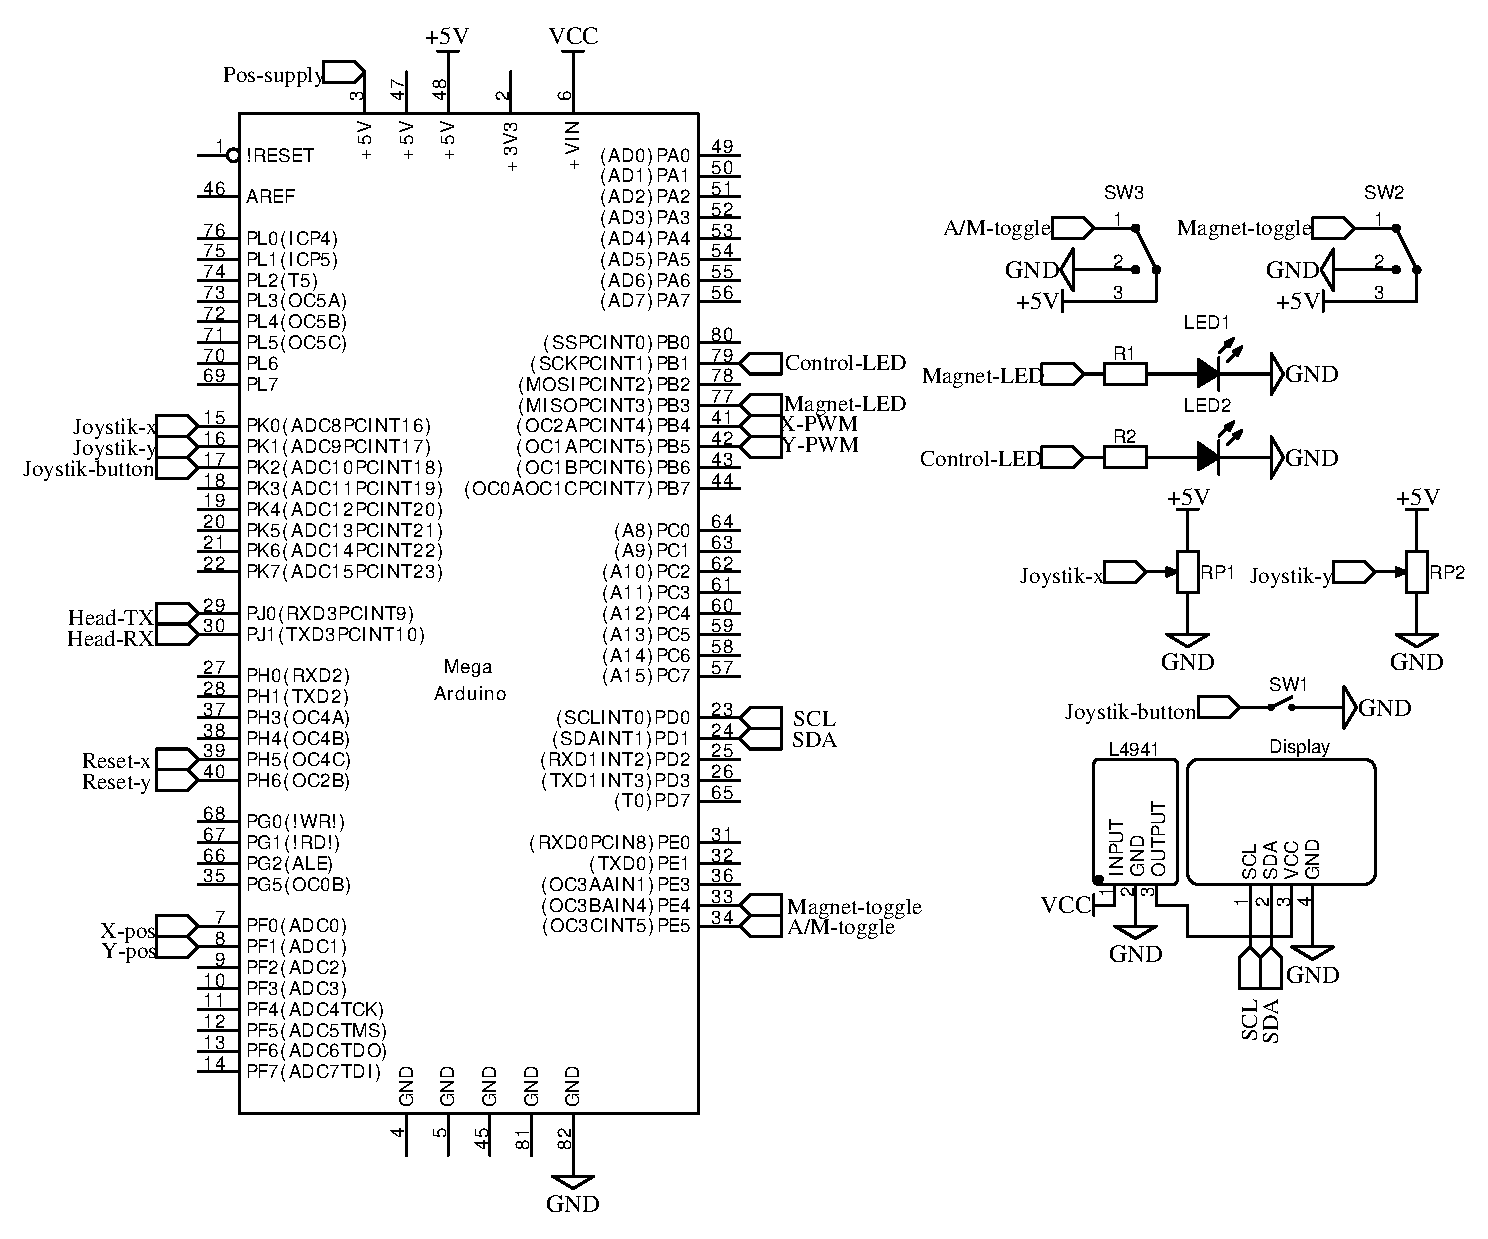
\includegraphics[width=1\textwidth]{pictures/Schematic_Kran_2022-02-16.pdf}
    \caption{Controller functional schematic.}
    \label{fig:controller_connections}
\end{figure}

\textbf{Links to hardware used:}\newline
L4941 \SI{5}{V} voltage regulator:\newline
\url{https://www.st.com/resource/en/datasheet/l4941.pdf}\\

Joystick:\newline
\url{https://www.amazon.com/SMAKN-Joystick-Breakout-Arduino-arduino/dp/B014MJLHC4}\\

\amega:\newline
\url{http://store.arduino.cc/products/arduino-mega-2560-rev3}\\

OLED screen:\newline
\url{https://dk.rs-online.com/web/p/oled-displays/2256197?cm_mmc=DK-PLA-DS3A-_-google-_-CSS_DK_DK_Displays_og_optoelektronik_Whoop-_-(DK:Whoop!)+OLED+displays-_-2256197&matchtype=&pla-302162021938&gclid=CjwKCAjw8sCRBhA6EiwA6_IF4cBCulk-WtMRrnzIQ23i7uNsbhB8FcUOVvLx726-mKff6_-QmLQVTRoCFzQQAvD_BwE&gclsrc=aw.ds}
\section{Controller software}\label{sec:controllerSoftware}

This section contains documentation of the controller software. The controller software contains the \texttt{manuel} function to control the crane manually, but has also been prepared for automated control with the \texttt{automated} function. It is possible to switch between the two functions using the switch built into the remote, where an LED is implemented to inform the user which function is selected. An LED is also used to indicate whether the switch to toggle the magnet has been press, and also to indicate whether the controller is being powered. The code for the controller is found via the following github link \url{linktilgit}

\subsection{Joystick data conversion}

As the joystick outputs two integers between 0 and 1023 for the x- and y-position, and the motor drivers for the x- and y-motor takes two PWM-signals with a duty cycle between \SI{10}{\%} and \SI{90}{\%} as inputs, a conversion is necessary. The Arduino has a function for generating PWM-signals named \texttt{analogWrite} which converts an integer between 0 and 255 to a \SI{5}{V} PWM-signal with a duty cycle between \SI{0}{\%} and \SI{100}{\%}. In order to linearly increase the PWM-signals from \SI{10}{\%} to \SI{90}{\%} using the \texttt{analogWrite} function, the linear function shown in equation \ref{eq:sec:systemDesign:linearPWM} is used.

\begin{equation}
    f(j_\text{val}) = 0.198 \cdot j_\text{val} + 26
    \label{eq:sec:systemDesign:linearPWM}
\end{equation}

\begin{table}[H]
    \begin{tabular}{l|l l l}
        $j_\text{val}$ & Value for the x- or y-position of the joystick & [-] \\
        \end{tabular}
\end{table}

\subsection{Deadzone calculator}

Two enable pins are used to turn off the x and y motor drivers, when the joystick is in the middle position. The joystick outputs 511 or 512 as x and y value, when being placed in the middle position. Therefore, the x enable pin is set to low when the value x-value of the joystick is between 510 and 513. Likewise, the y enable pin is set to low when the value y-value of the joystick is between 510 and 513.

\subsection{Software endstop}

A software end stop function is employed as a safety feature to ensure that the trolley or head does not exceed the operating area. The software endstop is employed as a function which takes the PWM-signal, minimum position, maximum position and current position as inputs. The functions returns the regulated PWM-signal, and can therefore be used to regulate both the head and the trolley of the crane. 

\begin{comment}
\subsection{Software}

The functionalities described above are implemented as a combined function as shown in figure \ref{fig:sec:systemdesign:manualControllerSoftware}. 

\begin{figure}[H]
    \centering
    \includegraphics[width = 0.7\textwidth]{pictures/manualControllerFunction (1).pdf}
    \caption{Manual control function.}
    \label{fig:sec:systemdesign:manualControllerSoftware}
\end{figure}

\begin{table}[H]
\centering
\begin{tabular}{|l|l|l|l|}
\hline
\rowcolor[HTML]{C0C0C0} 
Name                 & Functionality                 & Input & Output  \\ \hline
\texttt{endstop}              & Software endstop for x- and y & PWM, min, max, pos & PWM \\ \hline
\texttt{joystickOutputFormat} & Format joystick data          & joystickData & PWM \\ \hline
\texttt{joystickDeadZone}     & Determine deadzone            & joystickData & enableData \\ \hline
\texttt{toggleManual}         & Toggle manual control         & Bool & 0 or 5 V \\ \hline
\texttt{toggleMagnet}         & Toggle magnet                 & Bool & 0 or 5 V \\ \hline
\end{tabular}
\end{table}
\end{comment}
\end{document}



